% \chapter{議論と考察}
% 第4章では、RbのESR周波数シフト測定によって$^3$He偏極度の絶対値を求め、AFP-NMR法により得られるNMR信号強度の較正を行った。また第5章では$70~{\rm MeV}$の陽子ビームを用いた陽子--$^3$He弾性散乱実験による、有効散乱角度における$^3$He偏極分解能の測定を行った。$^3$He偏極分解能を求める際の$^3$He偏極度は、RbのESR周波数シフト測定により得られた較正結果から算出した。\\
%  本章では、これらの測定結果についての議論および考察、また今後の課題について述べる。

% %%%% 6.1 %%%%
%  \section{RbのESR周波数シフト測定の測定精度}
% 本研究では、$^3$He偏極度の絶対値を得るためにRbのESR周波数シフト測定システムを開発し、開発したシステムを用いて$^3$He偏極度測定を行った。$^3$He偏極度の測定精度としては$10$%以下を要請した。RbのESR周波数シフト測定によって得られたデータをフィッティングした結果、NMR信号強度$V_{\rm NMR}$に対する$^3$He偏極度$P_{\rm ^3He}$は、式(\ref{rel_P_3He-Vnmr})でも示したように
% %
% \begin{equation}
%  P_{\rm ^3He}~[%] = (5.72 \pm 0.61) \times 10^{-2} V_{\rm NMR}~[{\rm mV}]
%  \label{rel_P_3He-Vnmr2}
% \end{equation}
% %
% となった。フィッティングで得られた結果によると、およそ$11$%の精度で$^3$He偏極度が得られることが分かった。しかし、式(\ref{ESR_shift})のようにRbのESR周波数シフト$\Delta \nu_{\rm ESR}$は$^3$He偏極度$P_{\rm ^3He}$、$^3$Heの数密度$[{\rm ^3He}]$およびオーブン温度に依存する係数$\kappa_0$の積に比例する。フィッティングでは、$^3$Heの数密度$[{\rm ^3He}]$およびオーブン温度$T$の誤差を考慮していない。よって、ここではこれらの誤差を考慮した場合におけるRbのESR周波数シフト測定の測定精度について述べる。\\
%  $^3$He偏極度$P_{\rm ^3He}$を、NMR信号強度$V_{\rm NMR}$またはRbのESR周波数シフト$\Delta \nu_{\rm ESR}$の関数として
% %
% \begin{eqnarray}
%  P_{\rm ^3He}~[%] &\equiv& \alpha \times V_{\rm NMR}~[{\rm mV}]
%  \label{P-Vnmr} \\
%  &=& \beta \times \Delta \nu_{\rm ESR}~[{\rm kHz}]
%  \label{P-Delnu}
% \end{eqnarray}
% %
% と表すことにする。ここで、式(\ref{rel_P_3He-Vnmr2})のフィッティングの結果から$\alpha = 5.72$である。また$\beta$は
% %
% \begin{equation}
%  \beta = \frac{1}{C \kappa_0 [{\rm ^3He}]}
% \end{equation}
% %
% \begin{equation}
%  C = \frac{4\mu_0}{3} \frac{\mu_{\rm K} \mu_{\rm B} g_e}{h(2I+1)} \left( 1\mp \frac{8I}{(2I+1)^2} \frac{\mu_{\rm B} g_e B_0}{hA_{\rm hfs}} \right)
%  \label{C_beta}
% \end{equation}
% %
% である。ここで、式(\ref{C_beta})における括弧内の第二項は第一項に対して数%の寄与であるため、静磁場$B_0$の誤差は無視できるとした。$^3$Heの数密度$[{\rm ^3He}]$およびオーブン温度$T$の誤差、すなわち$\beta$の誤差$\delta \beta$を評価するために、式(\ref{P-Delnu})を
% %
% \begin{equation}
% P_{\rm ^3He}~[%] = \frac{\alpha}{\beta} \cdot \beta \times V_{\rm NMR}~[{\rm mV}]
% \label{P-Vnmr2}
% \end{equation}
% %
% と変形する。式(\ref{rel_P_3He-Vnmr2})におけるフィッティングによる誤差は、$\Delta \nu_{\rm ESR} = \alpha/\beta \times V_{\rm NMR}$より
% %
% \begin{equation}
%  \delta \left( \frac{\alpha}{\beta} \right) \beta = 0.61 \times 10^{-2}
% \end{equation}
% %
% と表される。また$\beta$の誤差$\delta \beta$は、$^3$Heの数密度$[{\rm ^3He}]$の誤差$\delta N_{\rm ^3He}$および$\kappa_0$の誤差$\delta \kappa_0$を用いて、誤差の伝播式から
% %
% \begin{eqnarray}
%  \delta \beta &=& \sqrt{\left( \frac{\partial \beta}{\partial [{\rm ^3He}]} \right)^2 (\delta N_{\rm ^3He})^2 + \left( \frac{\partial \beta}{\partial \kappa_0} \right)^2 (\delta \kappa_0)^2} \nonumber \\
%  &=& \beta \sqrt{\left( \frac{\delta N_{\rm ^3He}}{[{\rm ^3He}]} \right)^2 + \left( \frac{\delta \kappa_0}{\kappa_0} \right)^2}
%  \label{dbeta}
% \end{eqnarray}
% %
% となる。次に、$^3$Heの数密度$[{\rm ^3He}]$の誤差$\delta N_{\rm ^3He}$および$\kappa_0$の誤差$\delta \kappa_0$を求める。\\
%  $^3$Heの数密度$[{\rm ^3He}]$は、セル封入時のバラトロンゲージが示すガス圧力から求めた。この誤差$\delta N_{\rm ^3He}$として、バラトロンゲージの出力電圧値の読み取り誤差を$\delta V_{\rm bara}=0.01~{\rm V}$として考慮すると
% %
% \begin{equation}
%  \delta N_{\rm ^3He} = \frac{0.01}{1.513 \times 10^{-3}} \simeq 6.00 \times 10^{17}~[{\rm cm^{-3}}] 
%  \label{num_den_3He2}
% \end{equation}
% %
% となった。式(\ref{num_den_3He})より、$[{\rm ^3He}] = 8.17 \times 10^{19}~{\rm cm^{-3}}$であるから
% %
% \begin{equation}
%  \frac{\delta N_{\rm ^3He}}{[{\rm ^3He}]} = \frac{6.00 \times 10^{17}}{8.17 \times 10^{19}} \simeq 7.34 \times 10^{-3}
% \end{equation}
% %
% となる。また係数$\kappa_0$は式(\ref{kappa_0})でも示したように
% %
% \begin{equation}
%  \kappa_0 = 4.52+0.00934(T~[℃])
%  \label{kappa_02}
% \end{equation}
% %
% と表されるので、オーブン温度の誤差を$\delta T=2~$℃とすると$\kappa_0$の誤差$\delta \kappa_0$は
% %
% \begin{eqnarray}
%  \delta \kappa_0 &=& \sqrt{ \left( \frac{\partial \kappa_0}{\partial T} \right)^2 (dT)^2} \nonumber \\
%  &=& 0.00934 \times dT = 0.01868
%  \label{dkappa_0}
% \end{eqnarray}
% %
% となる。$T = 160~℃$とすると、式(\ref{kappa_02})より$\kappa_0 = 6.0144$なので
% %
% \begin{equation}
%  \frac{\delta \kappa_0}{\kappa_0} = \frac{0.01868}{6.0144} \simeq 3.10 \times 10^{-3}
% \end{equation}
% %
% となる。これらの値を式(\ref{dbeta})に代入することより、$\delta \beta$は
% %
% \begin{equation}
%  \delta \beta \simeq 1.97 \times 10^{-4}
% \end{equation}
% %
% と求められる。$\delta \beta$による式(\ref{P-Vnmr2})への寄与は$\alpha \cdot \delta \beta/\beta$と表されるので
% %
% \begin{equation}
%  \alpha \cdot \frac{\delta \beta}{\beta} \simeq 4.57 \times 10^{-4} \simeq 0.04 \times 10^{-2}
% \end{equation}
% %
% と計算される。これはフィッティングによる誤差に対して$8$%程度の大きさであり、RbのESR周波数シフト測定による$^3$He偏極度の測定誤差は、ESR周波数シフトの測定値の誤差が支配的であることが分かった。\\
%  これらの誤差を考慮すると、結局$^3$He偏極度とNMR信号強度$V_{\rm NMR}$との関係は
% %
% \begin{equation}
%  P_{\rm ^3He}~[%] = [5.72 \pm (0.61)_{\rm fit} \pm (0.04)_{\rm oth}] \times 10^{-2} V_{\rm NMR}~[{\rm mV}]
%  \label{rel_P_3He-Vnmr3}
% \end{equation}
% %
% となった。ここで、$\pm(0.61)_{\rm fit}$はフィッティングによる誤差であり、$\pm(0.04)_{\rm oth}$は$^3$Heの数密度$[{\rm ^3He}]$およびオーブン温度に依存する係数$\kappa_0$に起因する誤差である。よって、本研究において開発したRbのESR周波数シフト測定による$^3$He偏極度測定システムは、測定精度$11$%程度を達成していることが分かった。
% %%%%%%%%%%

% %%%% 6.2 %%%%
%  \section{$^3$He偏極分解能$A_y$の測定精度}
% 東北大学CYRICで行った$70~{\rm MeV}$の陽子--$^3$He弾性散乱実験によって、$^3$He偏極分解能$A_y$は式(\ref{Ay_result_55})および式(\ref{Ay_result_70})でも示したように
% %
% \begin{eqnarray}
%  A_y(\theta_{\rm lab} = 55^{\circ}) &=& -0.35 \pm (0.01)_{\rm stat}
%  \label{Ay_result_55_2} \\
%  A_y(\theta_{\rm lab} = 70^{\circ}) &=& -0.33 \pm (0.03)_{\rm stat}
%  \label{Ay_result_70_2}
% \end{eqnarray}
% %
% と得られた。ここでは、統計誤差のみを示した。以下では、$^3$He偏極分解能$A_y$の系統誤差について考察する。\\
%  系統誤差としては、主に以下の二つが考えられる。
% %
% \begin{enumerate}
%  \item RbのESR周波数シフト測定による$^3$He偏極度の測定精度に起因する系統誤差$(\delta A_y)_{\rm pol}$
%  \item 本実験における散乱測定系の系統誤差$(\delta A_y)_{\rm sca}$
% \end{enumerate}
% %
%  1.については、6.1節で述べたように本研究で開発したRbのESR周波数シフト測定による$^3$He偏極度測定システムにおける測定精度は$11$%程度であるから、それによる$^3$He偏極分解能$A_y$の系統誤差$(\delta A_y)_{\rm pol}$も、$^3$He偏極分解能測定で得られた値に対して$11$%程度となる。\\
%  2.については、散乱実験時のビームの状態や検出器系の系統誤差等、様々な要因が寄与してくるため見積もることが困難である。そこで、この散乱測定系での系統誤差を評価するために、非偏極状態の$^3$He標的を用いた散乱の擬非対称度測定を行った。$^3$He偏極度が$0$%であれば、ビーム方向に対して左右に設置した検出器における陽子--$^3$He弾性散乱イベントの検出数は等しくなる。また、$^3$He核スピンの向き対しても検出数は等しくなるはずである。この非偏極$^3$He標的を用いた測定において非対称が確認されれば、その大きさが散乱測定系の系統誤差になると考えられる。\\
%  擬非対称度測定の結果、実験室系での散乱角度$55^{\circ}$および$70^{\circ}$に設置した左右のそれぞれの検出器において
% %
% \begin{eqnarray}
%  |(p_y \cdot A_y)_0| &=& \left| \frac{L_{\rm up}-L_{\rm down}}{L_{\rm up}+L_{\rm down}} \right| = \left| \frac{R_{\rm down}-R_{\rm up}}{R_{\rm up}+R_{\rm down}} \right| \nonumber \\
%  &\sim& 0.01
% \end{eqnarray}
% %
% 程度の非対称度が得られた。左辺の添え字の0は非偏極状態を表す。よって、散乱測定系の系統誤差$(\delta A_y)_{\rm sca}$は
% %
% \begin{equation}
%  (\delta A_y)_{\rm sca} = \frac{|(p_y \cdot A_y)_0|}{p_y} \simeq 0.1
% \end{equation}
% %
% となり、偏極$^3$He標的を用いた$^3$He偏極分解能測定で得られた値に対しておよそ$30$%程度と求められた。以上の結果から、$^3$He偏極分解能$A_y$の誤差は、系統誤差が支配的であることが分かった。\\
%  本研究において得られた$^3$He偏極分解能$A_y$と、二体核力ポテンシャルによる理論計算\cite{Del_pra}とを比較した結果を図\ref{Ay_comp_2NF}に示す。図\ref{Ay_comp_2NF}では、二体核力ポテンシャルによる理論計算を赤線で示している。また測定した$^3$He偏極分解能の統計誤差を棒付きのエラーで、散乱測定系の系統誤差を括弧のエラーで示している。本実験で得られた$^3$He偏極分解能は系統誤差が大きく、誤差の範囲以上の二体核力ポテンシャルによる理論計算値との差は見られない。三体核力の効果について詳細に調べるためには二体核力ポテンシャルによる理論計算値と高精度の$^3$He偏極分解能の測定値との比較が必要である。故に三体核力の効果について議論を行うためには、$^3$He偏極分解能の系統誤差の抑制が求められる。

% \begin{figure}[tbp]
%  \centering
%  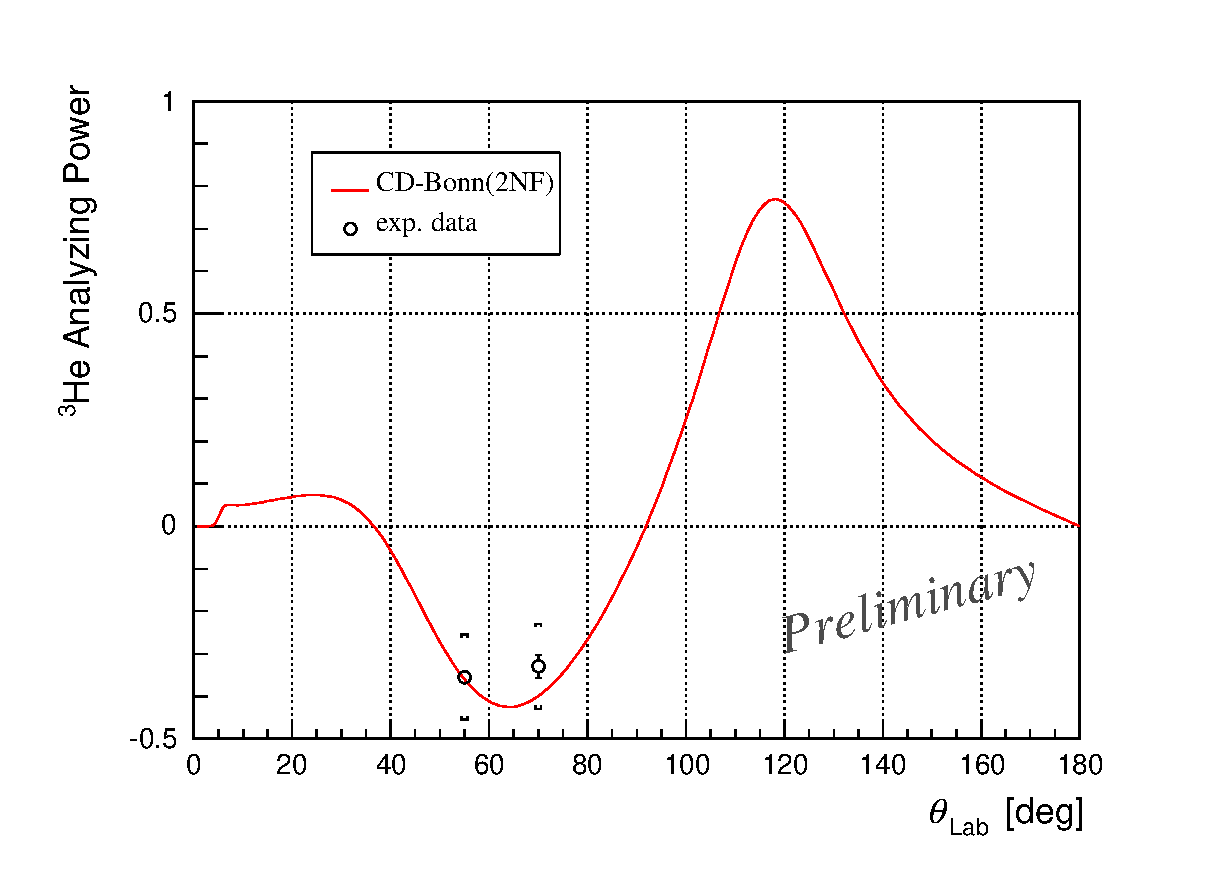
\includegraphics[clip, width=11cm]{./chap6/fig/Ay_calc_CDBonn3.eps}\\
%  \caption{$70~{\rm MeV}$の陽子--$^3$He弾性散乱における$^3$He偏極分解能の測定結果および二体核力ポテンシャルによる理論計算}
%  \label{Ay_comp_2NF}
% \end{figure}


% %%%%%%%%%%

% %%%% 6.3 %%%%
%  \section{$^3$He偏極分解能の測定精度の向上}
% 前節で述べたように、本実験において得られた$^3$He偏極分解能$A_y$の誤差は、系統誤差が支配的であることが明らかとなった。$^3$He偏極分解能を高精度で測定するためには、系統誤差の抑制が要請される。\\
%  散乱測定系の系統誤差に関しては、偏極$^3$He標的の偏極度が向上すれば相対的に小さくすることが出来る。$^3$He偏極度を向上させるために、光ポンピングに用いる半導体レーザーの高出力化および狭帯域化を計画している。本研究において用いた半導体レーザーの線幅は$2~{\rm nm}$程度であり、$3$気圧の$^3$Heガス存在化でのRbの吸収線幅である$54~{\rm GHz}$に対して非常に大きい。狭帯域化および高出力化を図ることによって、Rb原子の偏極生成効率を飛躍的に向上させ、結果的に$^3$He偏極度を向上させることが期待される。またガラスセル製作時の洗浄方法を見直し、標的セル内の不純物を抑制することでも更なる$^3$He偏極度の向上が期待される。\\
%  系統誤差の抑制には、本研究で開発したRbのESR周波数シフト測定による$^3$He偏極度測定システムの測定精度の向上も要請される。測定誤差の要因としては、RbのESR周波数シフト測定中での静磁場の揺らぎが考えられる。本研究ではフィードバック回路を組み込むことによって振動磁場の周波数が常に共鳴周波数付近に変調されるようにしたが、静磁場の揺らぎによる補正も必要である。そこで、今後は高精度のフラックスゲート磁力計を用いた磁場測定をRbのESR周波数シフト測定中に行うことによって、静磁場の揺らぎの補正を考慮する方針である。またガラスセルに封入した$^3$Heガスは、時間経過と共にガラスを透過していってしまう。よって、ガスの封入時に測定した$^3$Heガスの圧力、すなわち$^3$Heの数密度は次第に減少していくことになる。$^3$Heの数密度を正確に得るためには、ガラスセルへの封入後に$^3$Heガスの圧力を測定するためのシステムの構築が求められる。$^3$Heガス圧力の測定方法としては、Rbの吸収スペクトルが混合気体である$^3$Heガスの圧力によって拡がる現象を利用した圧力拡がり測定がある。今後は、この測定システムを導入し、RbのESR周波数シフト測定による$^3$He偏極度測定システムのさらなる測定精度の向上も視野に入れている。


% %%%%%%%%%%